\subsubsection*{A5.8}
\subsubsection*{(a)}
\paragraph{}
We can write it into a convex optimization form with
\begin{align*}
A=\begin{bmatrix*}[r]
g(t_1)^T\\ 
g(t_2)^T\\
... \ \ \\
g(t_N)^T
\end{bmatrix*}
\text{,} \quad 
b=\begin{bmatrix*}[r]
y_1\\ 
y_2\\
... \\
y_N
\end{bmatrix*}
\end{align*}
\paragraph{}
To guarantee that $x^Tg(t)$ is convex in t on $[\alpha_0,\alpha_M]$, because the cubic spline is piece-wise polynomial, its second derivative is piece-wise linear and therefore $f''(t) \geq 0$ on $[\alpha_0,\alpha_M]$ if $f''(t) \geq 0$ for $t=\alpha_0,\ \alpha_1,...,\alpha_M $. Therefore
\begin{align*}
G=-\begin{bmatrix*}[r]
g''(\alpha_0)^T\\ 
g''(\alpha_1)^T\\
... \ \ \\
g(\alpha_M)^T
\end{bmatrix*}
\end{align*}
\subsubsection*{(b)}
\paragraph{}
See the following figure and M-code:
\begin{figure}[h]
	\centering
	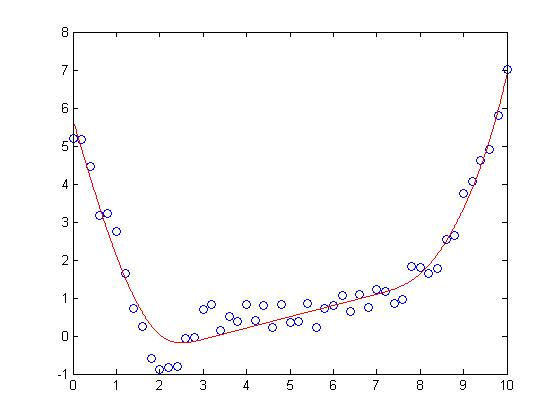
\includegraphics[scale=0.5]{cubicfit}
	\caption{Cubic spline fit with convex constraint}
\end{figure}
\verbatiminput{cubic_spline_main.m}


